\documentclass[a4paper, 12pt]{article}
\usepackage{graphicx} % Required for inserting images
\usepackage{fullpage}
\usepackage{amsmath}
\usepackage{xcolor}
\usepackage{float}
\usepackage{geometry}
\usepackage{biblatex}
\geometry{margin=1in}
\usepackage{enumitem}
\usepackage{hyperref}
\usepackage{microtype}
\usepackage{amsmath}
\usepackage{parskip}

\title{02-09-25 Mean, Median, Mode}
\author{C\&L Math Tutoring}
\date{February 9, 2025}

\begin{document}

\maketitle

\subsection*{Measures of Central Tendency}
Mean, median, and mode are all \textbf{measures of central tendency.} They each tell you something important about the data that you're analyzing.

\subsubsection*{Mean}
The \textbf{mean}, also called the average, is calculated by \textcolor{blue}{adding all terms together and then dividing by the total number of terms.}

The mean would be a better measure of central tendency when the data is symmetrical.

$$\text{Mean} = \frac{\text{sum of all terms}}{\text{number of terms}}$$

\subsubsection*{Median}
The \textbf{median} is the \textcolor{blue}{middle number in a set of terms when they are put in order.} If there are 2 middle numbers (even number of terms), you would add them together and divide by 2.

The median would be a better measure of central tendency when the data is skewed left/right (not symmetrical).

\subsubsection*{Mode}
The \textbf{mode} is the \textcolor{blue}{number that appears the most in the set.}

Example: Anna takes 3 tests. She gets 100\%, 8\%, and 55\%. Find the mean, median, and mode of her scores.

Mean: $\frac{163}{3} \approx 54.33 $\\
Median: 55\% \\
Mode: n/a

\begin{figure}[H]
    \centering
    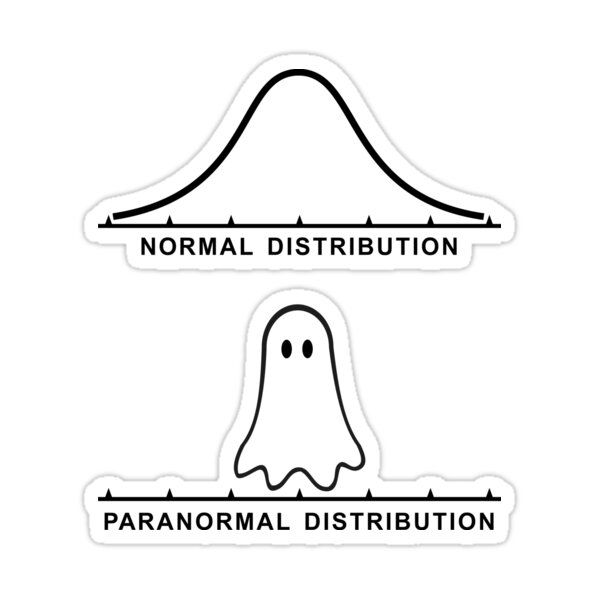
\includegraphics[width=0.5\linewidth]{meme.jpg}
    \label{fig:enter-label}
\end{figure}


\end{document}
